\subsection{Precision energy loss}\label{sec:preceloss}
One of the classic observables to measure the out-of-cone radiation due to jet quenching is the jet nuclear modification factor $R_{\mathrm{AA}}$. Measurements of the jet $R_{\mathrm{AA}}$ at the LHC have shown a suppression of a factor of two over a wide range of jet transverse momentum. Figure \ref{fig:jetRAA} shows the current precision (run2 statistics) and what can be achieved at the HL-LHC with a factor of 10 more data. Especially at high transverse momentum a strong reduction of the experimental uncertainties is expected which will allow a detailed study of the momentum dependence of the out-of-cone radiation. The jet $R_{\mathrm{AA}}$ is sensitive to various physics mechanisms such as color coherence and flavor dependence of energy loss. Models incorporating these various physics effects can be confronted with the high precision data from HL-LHC with as goal to determine what the relative contribution of each of these phenomena is. In addition to the inclusive jet $R_{\mathrm{AA}}$ it is particularly interesting to study the mid- and forward rapidity region separately since it allows to study the interplay between flavor and spectral steepness, and the path length dependence of jet quenching. As can be observed in the right panel of Fig. \ref{fig:jetRAA} especially in the high momentum region the rapidity dependence is strongest. This region will be accessible for the first time with high enough precision at the HL-LHC.
\begin{figure}[!ht]
\begin{center}
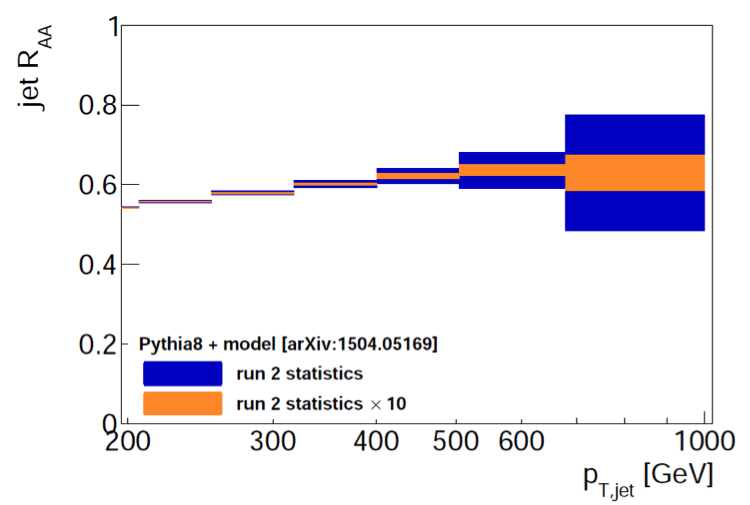
\includegraphics[width=.45\textwidth]{\main/jets/figures/atlas/ATLASJetRAAVsPtProjection.png}
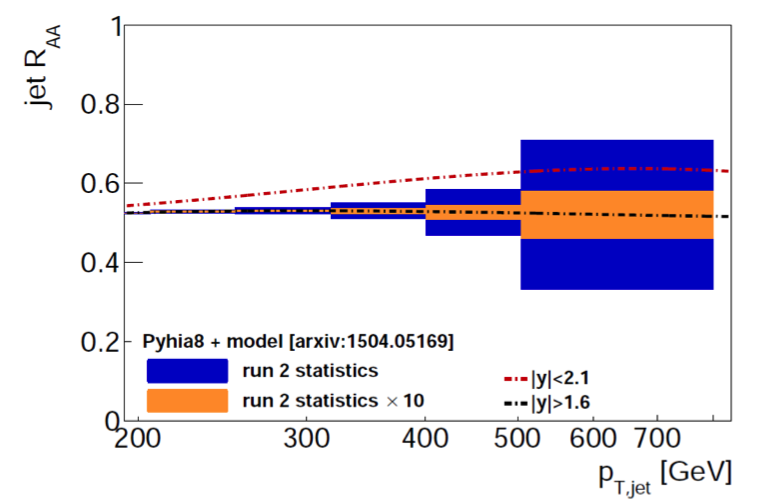
\includegraphics[width=.45\textwidth]{\main/jets/figures/atlas/ATLASJetRAAVsPtEtaBinsProjection.png}
\caption{Projection of the precision that can be reached for jet $R_{\mathrm{AA}}$ at the HL-LHC using calorimeter jets at ATLAS. [REF TO ATLAS NOTE]}
\label{fig:jetRAA}
\end{center}
\end{figure}

One of the most promising channels to study the parton energy loss mechanism are boson tagged jets. The bosons (photons or Z$^{0}$ bosons) escape the region of the hot dense medium unmodified. This has been confirmed through the absence of significant modification of both photon and Z$^{0}$ boson production in PbPb collisions relative to the binary collision-scaled pp baseline by both ATLAS and CMS collaborations \cite{Aad:2012ew,Aad:2015lcb,Chatrchyan:2012vq,Chatrchyan:2014csa}. However, the parton shower recoiling from the boson gets modified in heavy ion collisions due to the elastic and inelastic interactions with the QCD medium. Furthermore, jets produced opposite to the isolated boson
are more likely to originate from quarks, while dijet and hadron+jet correlations usually involve significant gluon fractions. 
Comparing Z+jet and $\gamma$+jet observables to dijets~\cite{Chatrchyan:2011sx,Chatrchyan:2012nia} (or hadron+jets \cite{Adam:2015doa}) will allow the studies of quark and gluon initiated jets probing the flavor dependence of jet quenching. Figures~\ref{fig:photonjet} and \ref{fig:Zjet} show the expected performance at the HL-LHC for the transverse momentum balance between the jet and the boson. The central values are based on the smoothed data from the previous CMS publications~\cite{Sirunyan:2017jic,Sirunyan:2017qhf}. The systematic uncertainties are reduced by a factor of two with respect to the results with the 2015 PbPb data due to the improvements on the jet energy scale and jet energy resolution uncertainties with the larger data sample at the HL-LHC. The collected number of $\gamma$+jet events will also be sufficient to study the path length dependence of jet quenching by performing measurements as a function of the reaction plane for the first time. In addition to the smaller uncertainties due to the enhanced statistics at the HL-LHC, it will also be possible to utilize higher momentum photons and Z$^{0}$ bosons allowing to measure larger energy losses. The LHC experiments also envision extending the low jet momentum reach allowing to recover those heavily quenched jets which currently are typically not selected for the measurement due to a limitation on the jet energy resolution. The jet resolution can be improved by using more sophisticated techniques for the background subtraction as was recently shown in Ref. \cite{Haake:2018hqn}.

\begin{figure}[!ht]
\begin{center}
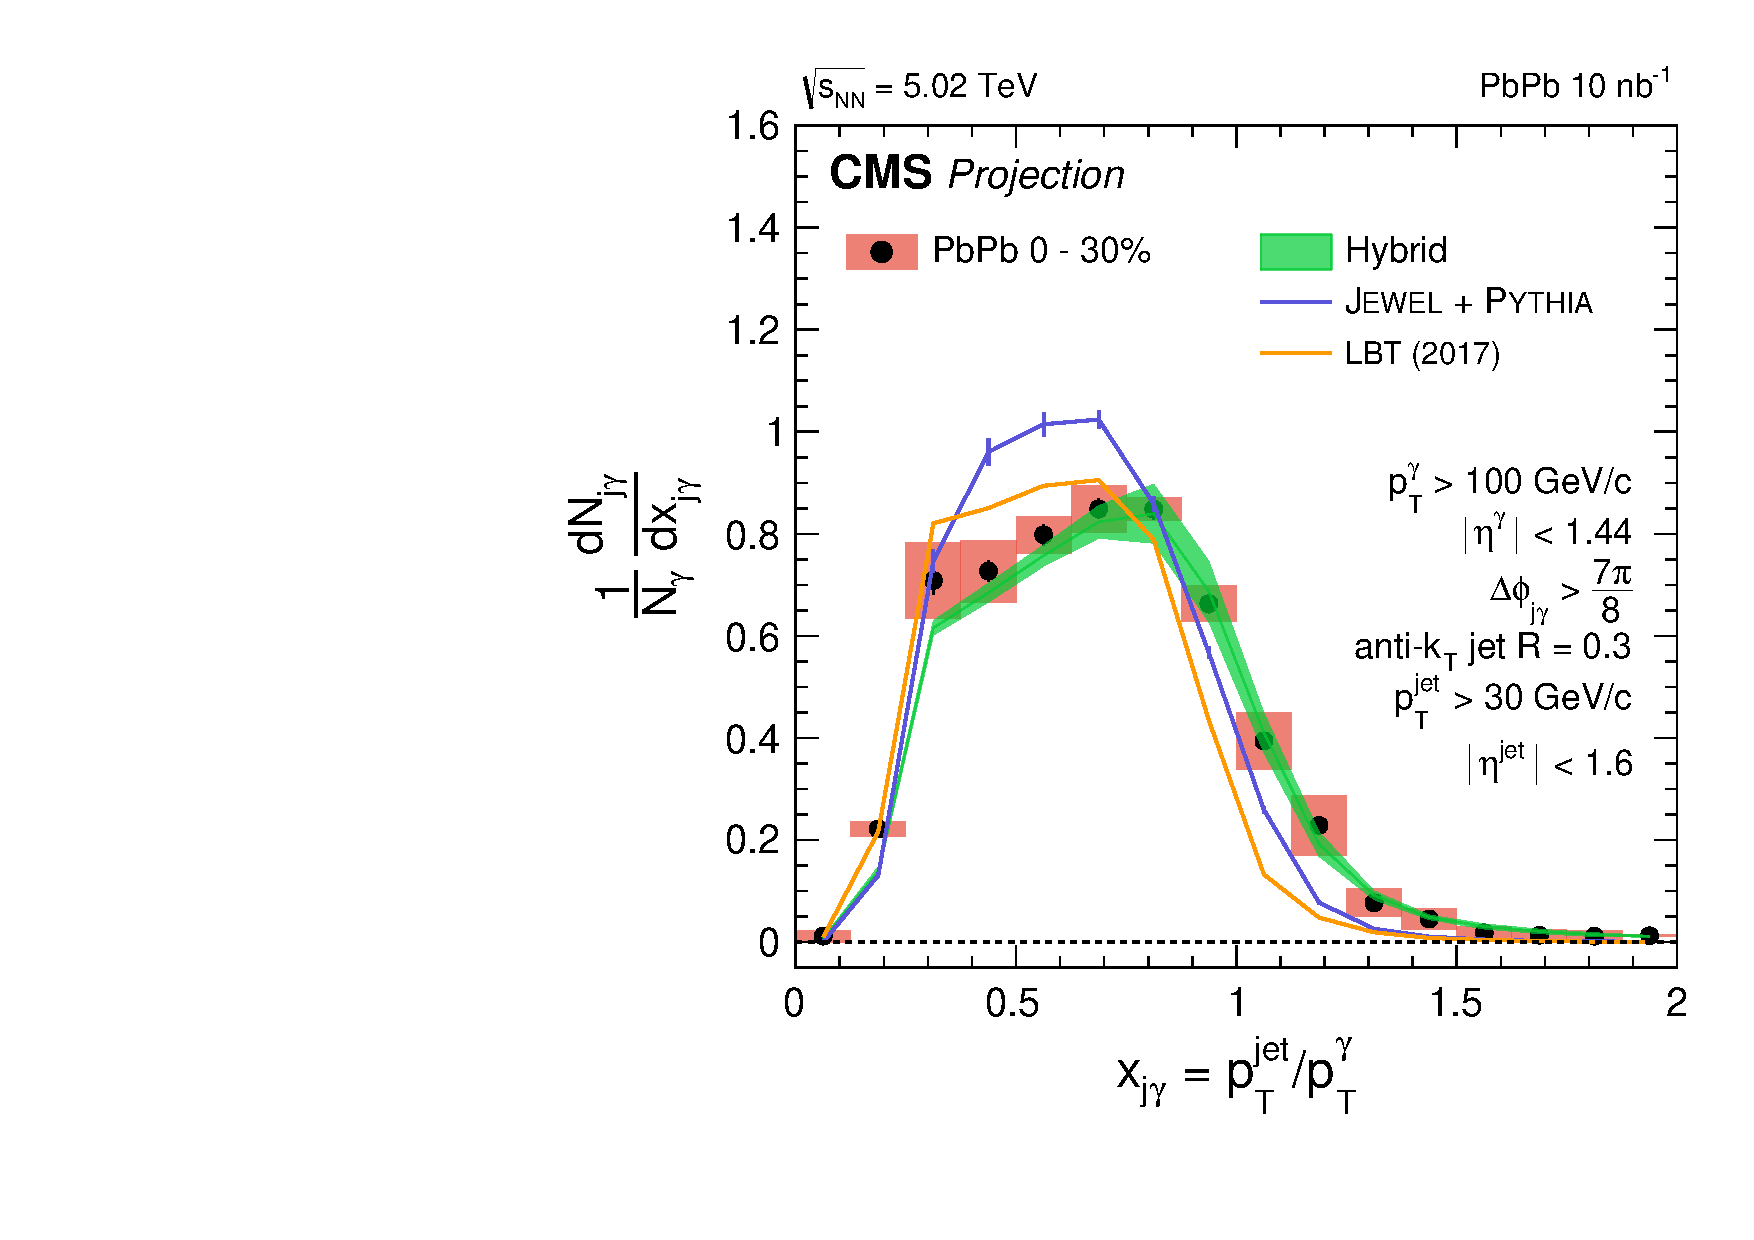
\includegraphics[width=.45\textwidth]{\main/jets/figures/cms/xjg_projection_2.pdf}
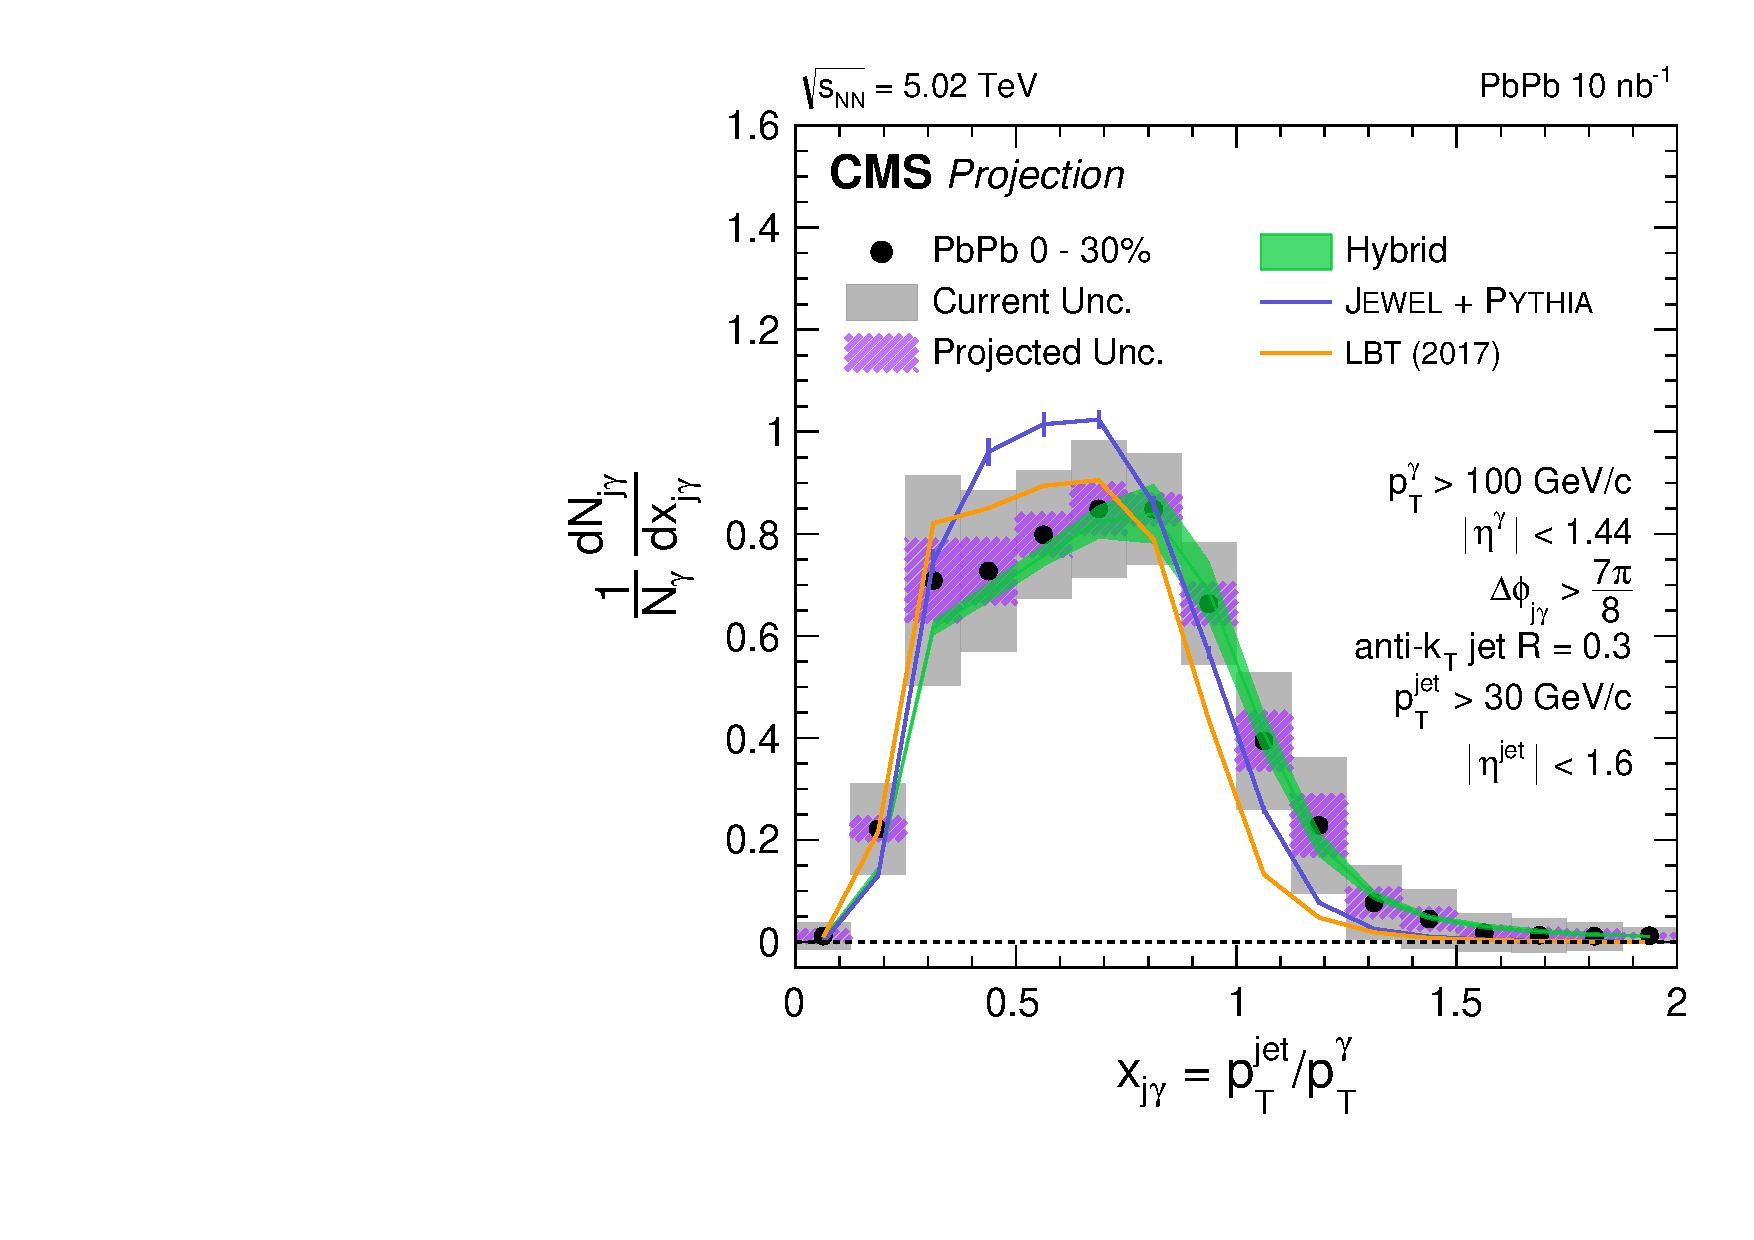
\includegraphics[width=.45\textwidth]{\main/jets/figures/cms/xjg_projection.pdf}
\caption{(Left Panel) $X_{j\gamma}$ distribution for isolated-photon+jets of $p_{\gamma}$ $> $ 100 GeV/c and $|\eta_{\gamma}|<1.44$, $p_{\rm jet} > $ 30 GeV/c and $|\eta_{\rm jet}| < 1.6$ in the HL-LHC data (Right Panel) Comparison between the current performance with 0.4 nb$^{-1}$ of PbPb data collected in 2015 and with HL-LHC data. \cite{CMS-FTR-17-002:2017dec}}
\label{fig:photonjet}
\end{center}
\end{figure}

\begin{figure}[!ht]
\begin{center}
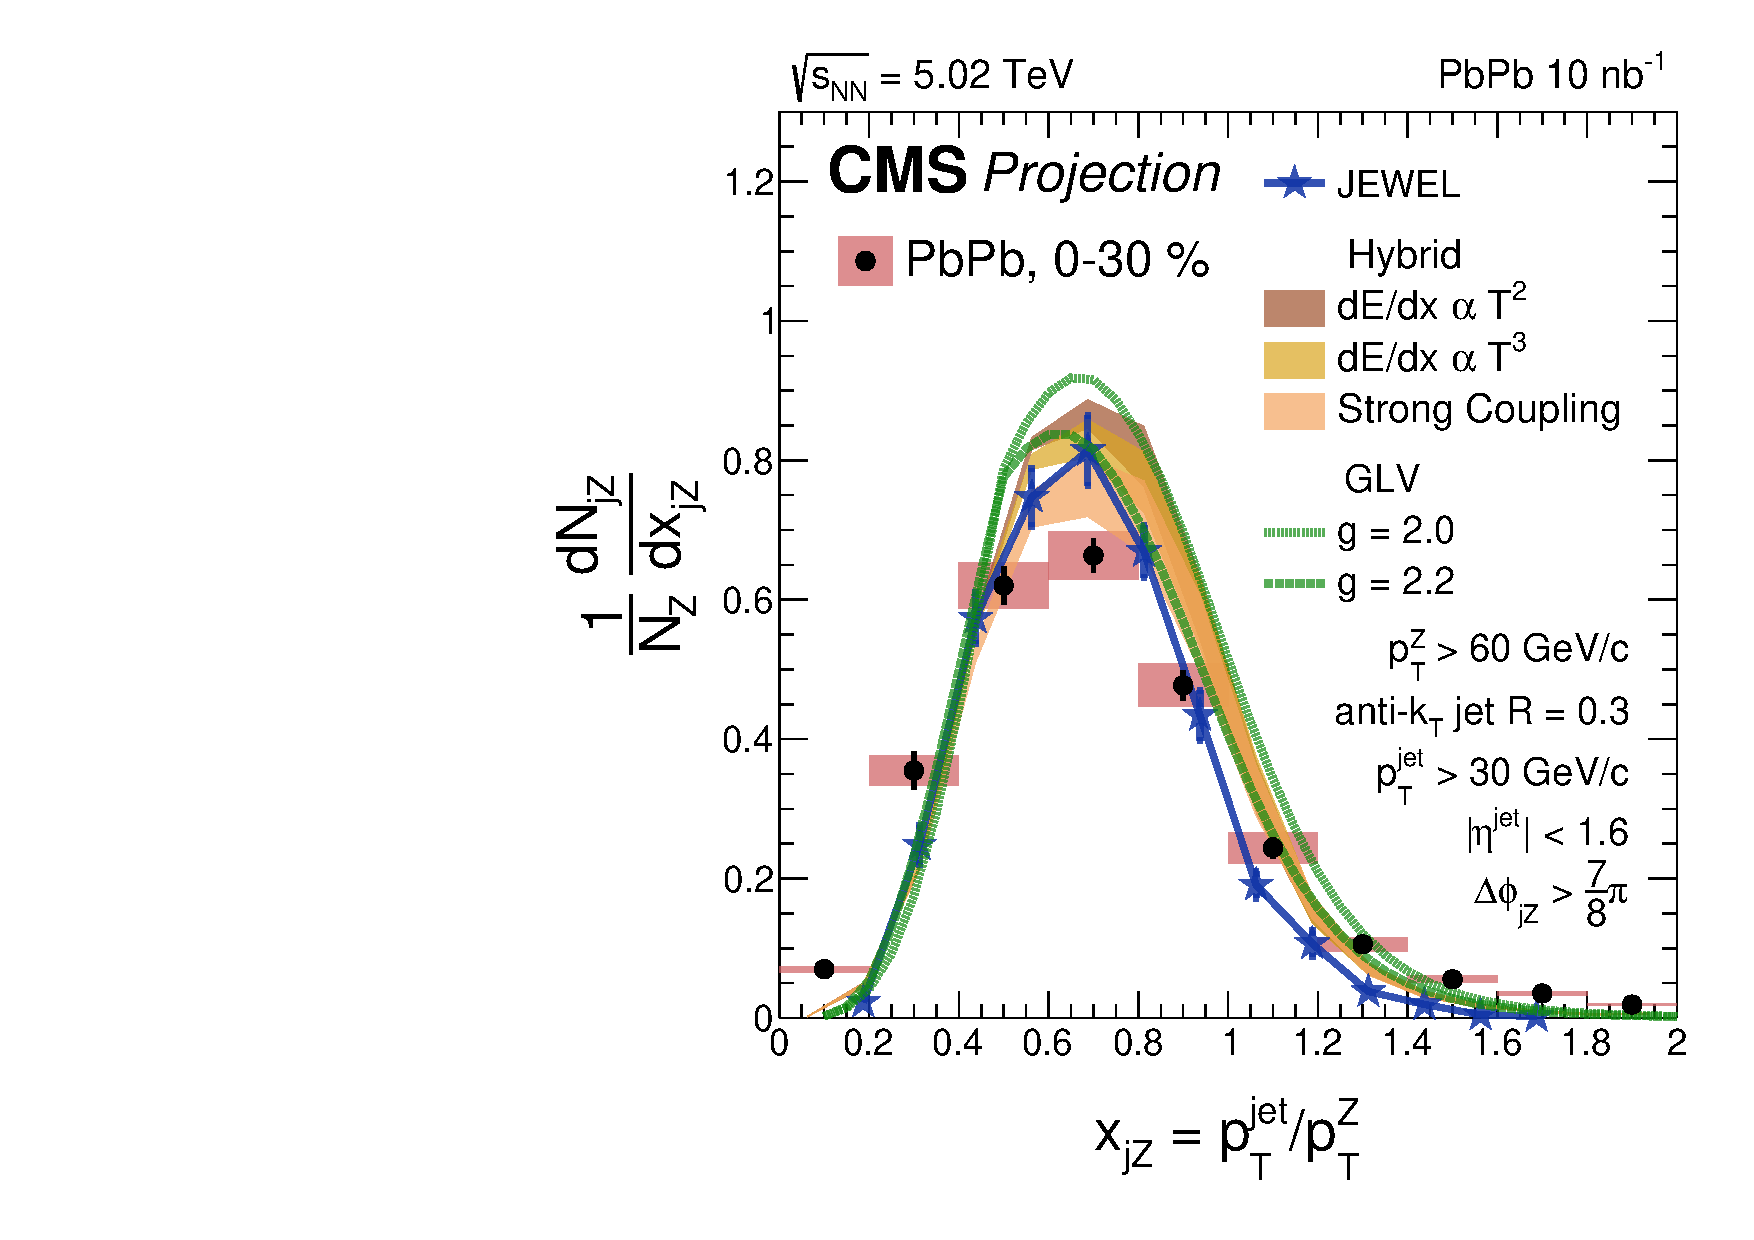
\includegraphics[width=.45\textwidth]{\main/jets/figures/cms/projection_xjz_Theory_sysReduced50Prct.pdf}
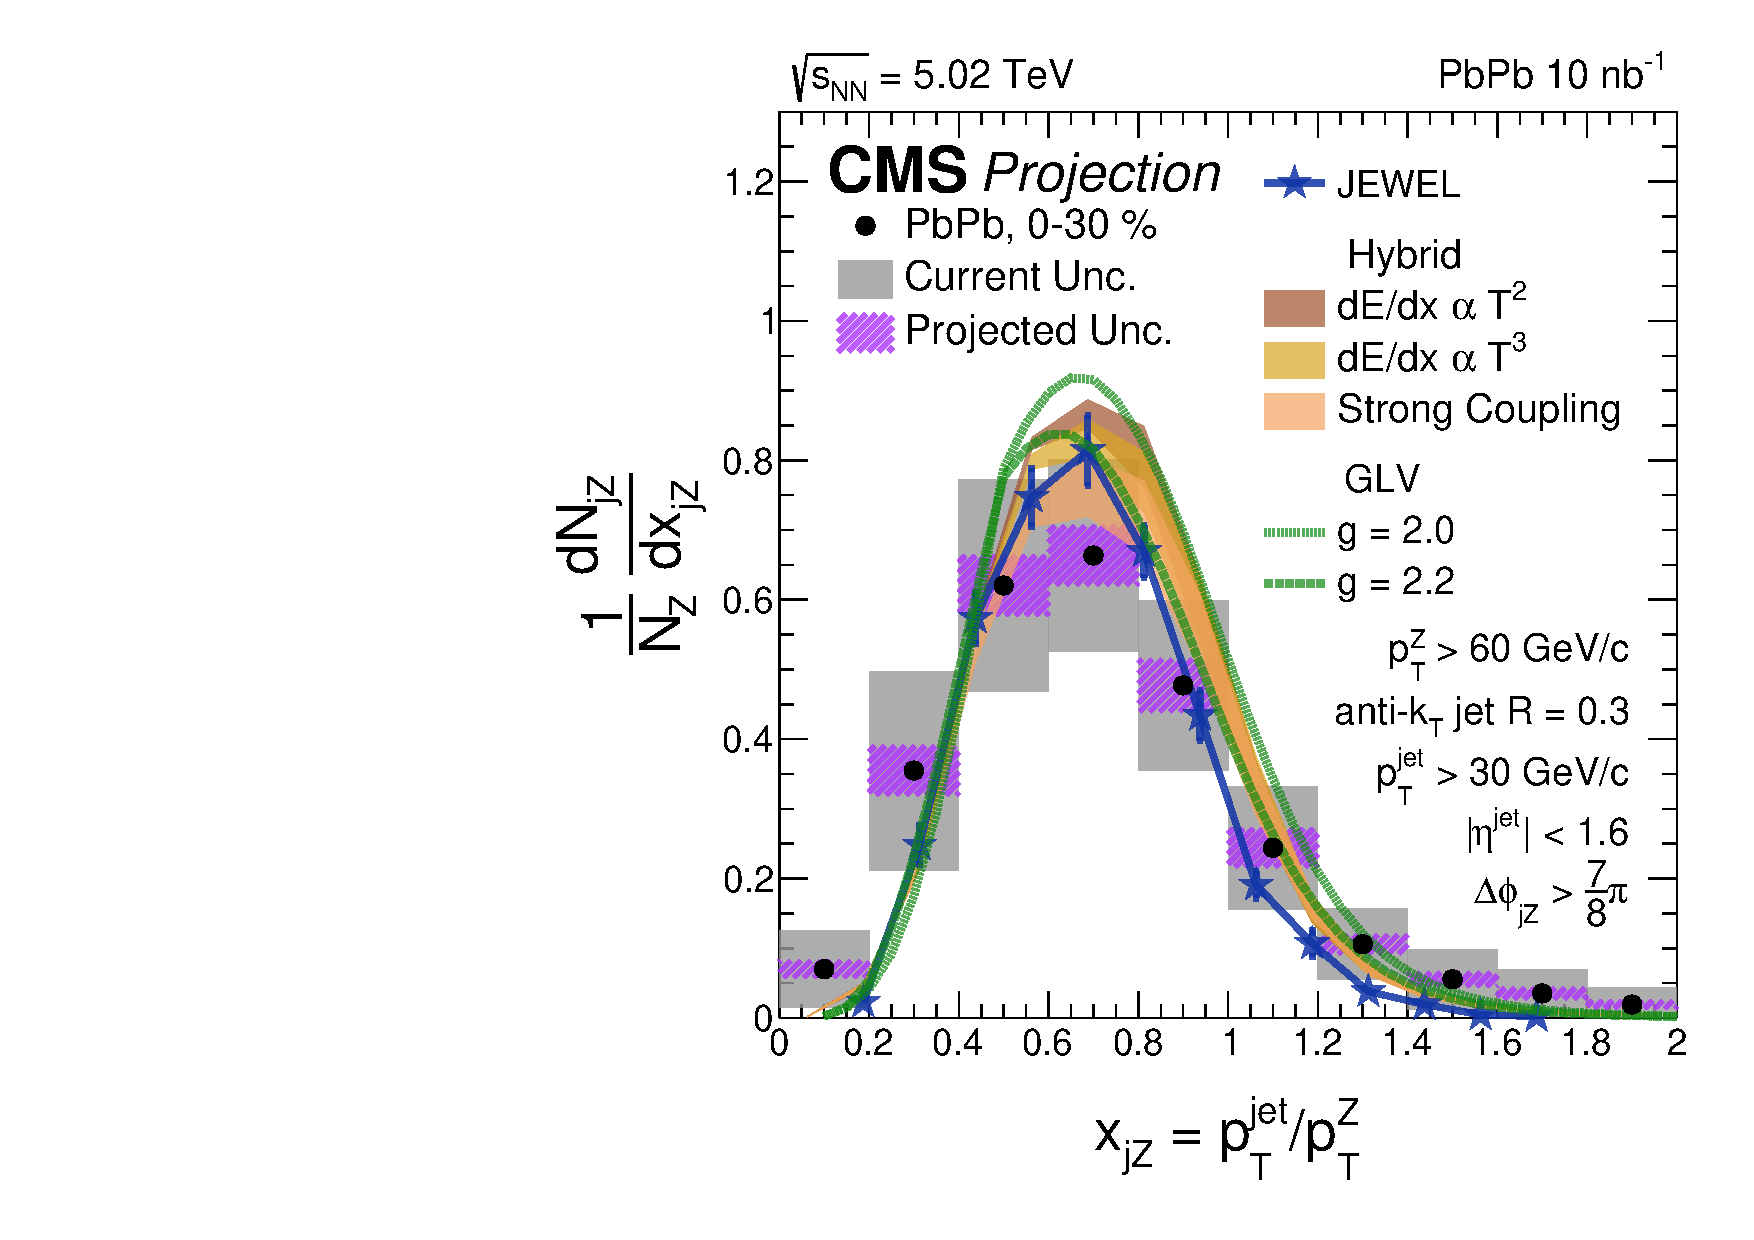
\includegraphics[width=.45\textwidth]{\main/jets/figures/cms/projection_xjz_Theory_MergedUnc_sysReduced50Prct.pdf}
\caption{(Left Panel) $X_{jZ}$ distribution for isolated-photon+jets of $p_{Z}$ $> $ 100 GeV/c, $p_{\rm jet} > $ 30 GeV/c and $|\eta_{\rm jet}| < 1.6$ in the HL-LHC data (Right Panel) Comparison between the current performance with 0.4 nb$^{-1}$ of PbPb data collected in 2015 and with HL-LHC data. \cite{CMS-FTR-17-002:2017dec}}
\label{fig:Zjet}
\end{center}
\end{figure}
